In this chapter, the visualization of objects whose positions have previously been computed (see Section ~\ref{ch:computation}) will be discussed. Also, the interaction patterns for the mobile application prototype will be defined.

\begin{itemize}
	\item \textbf {Visualization} - Describes how visualization is implemented in the App prototype.
	\item \textbf {User Interaction} - Lists information segments in the App prototype and possibilities of interaction for the user.
	\item \textbf {Removal of Node Overlapping} - Sketches the algorithm of how overlapping between multiple artist nodes are removed.
\end{itemize}

\section{Visualization}

After the computation of similarity measures and the resulting layout of music objects has been performed (see Section ~\ref{ch:computation}), the mode of visualization for the App prototype has to be defined. As has already been discussed, the possible modes of information display have been narrowed down due to several constraints, determining that a 2D visualization represents the best compromise for the scope of this thesis. Small screens on mobile devices introduce a further constraint: in most use cases, not all of the content will fit on one screen; therefore, a zooming and panning mechanism will be employed. To provide users with a rich experience, the objects shall not be shown as points, but as shapes - if an image of the object exists in an online source, it shall be used, or otherwise, a monocolored rectangle shall be shown. In order that users can orient themselves better, a non-solid background will be used - this provides visual feedback to the user while zooming when no objects are currently visible on the screen.

\begin{figure}[H]
  \centering
    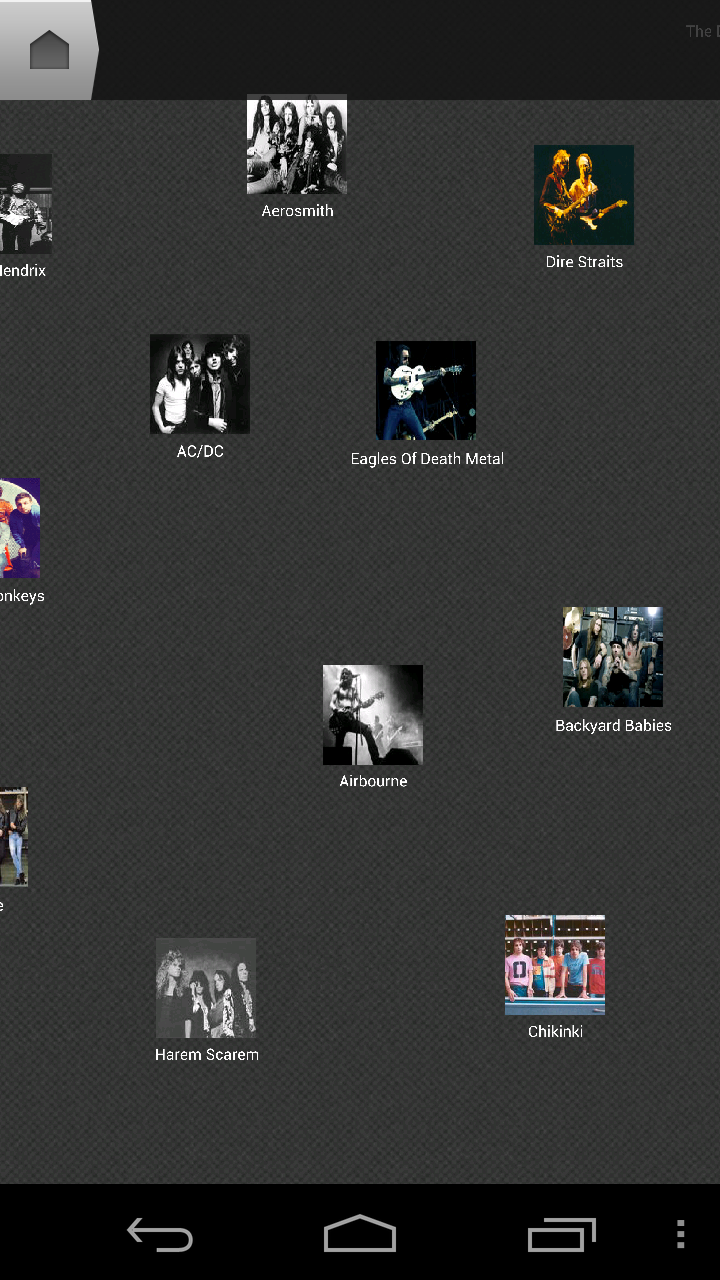
\includegraphics[width=0.4\textwidth]{figures/screen_mds_10_after_all_uncollided_nodes}
  \caption{Prototype Screenshot}
  \label{fig:prototype_screenshot}
\end{figure}

To let the reader grasp the previously described visualization, a screenshot of the prototype app is provided in Figure ~\ref{fig:prototype_screenshot}.

\section{User Interaction}

Information will be displayed to the user in a hierarchical way in the App prototype - to limit the amount of information displayed all at once, it is split up and logical links are established. The hierarchy is made up of:

\begin{itemize}
	\item \textbf{Artists} - images and labels with the names of the respective artists are displayed. Their positions relative to each other depict the artists' similarities. Here, the user can select an artist and proceed to the next hierarchical level by pressing a button:
	\item \textbf{A certain artist and her album(s)} - images and labels of the previously selected artist and her albums (stored on the device), arranged in a starlike way (without any similarity information conveyed). Again, the user can select an album and proceed to the next hierarchical level by pressing a button:
	\item \textbf{An album's tracks} - a list of tracks, carrying the image of the belonging album. The user can choose to start playback of one or all of the tracks.
	\item \textbf{Related Artists (Discovery)} - From within the \textbf{Artists} view, the user can choose to display artists which are related to a certain seed artist in a semantic way, as established by the Last.fm API. The newly retrieved related artists are added to the normal "'Artists"' view, by applying a dark, semitransparent overlay to the previously shown artists and background, and on top of that showing the related artists. The force-directed layout then starts to push the newly added related artists into a star-shaped array around the seed artist, and the user can either cancel discovery (removing the newly added related artists and the semitransparent overlay), or continue discovery (selecting a related artist and using it as an additional seed node is possible).
	
\end{itemize}


To improve the user's understanding of the current navigational status, so-called breadcrumbs are introduced. The user can navigate within a two level hierarchy, where the higher level shows artists, and the lower level allows the user to view the albums of a previously selected artist. Breadcrumbs achieve "'visitor location awareness in a simple and direct way"' \cite{Tesoriero:2008:Breadcrumbs} if applied to 2D spaces. A breadcrumb in this context is a series of links displayed on top of the graph, each representing one hierarchical level. An example for breadcrumbs shown while a list of tracks (lowest hierarchical level) could be: "'Artist: Air > Album: Talkie Walkie"'. Further, a button is added which positions the viewport at the center of the graph, for the user to recover in case she has lost track of the viewport's position.

Within the graph viewport, interaction will be a mix of touch based interaction and hardware/software buttons, since most Android devices provide those affordances. Special accessibility functions for interaction without touch gestures are omitted since they would go beyond the scope of this thesis.
Following the established conventions of touch interfaces, controllable objects (like artists or albums) are made touchable. Likewise, the user can reach upper view hierarchies by pressing the back button.
Exploration of the graph is performed by two common touch gestures, namely pinch-to-zoom and one-finger-panning. To zoom, the user places two fingers on the graph viewport and moving her fingers either apart (zooming in) or towards each other (zooming out). To pan, the user places one finger on the graph and moves it around as if it were a piece of paper and the screen an aperture showing the paper.

\section{Summary}

This chapter has made the concepts for visualization in the App prototype accessible to the reader. Apart from the introduction of implementation details regarding visualization (2D canvas for graph display, shape-based node rendering), the way how users interact with the prototype has been defined. Information is segmented into several contexts, "'breadcrumbs"' help the user navigate, and well-established multitouch gestures let the user control information presentation. 

As an improvement to readability and understandability of graph layouts, a computational method similar to force-transfer algorithms has been included in order to remove graph node overlappings.